%\documentclass[letterpaper,twocolumn,10pt]{article}
%\documentclass{sigcomm}
\documentclass{sig-alternate-10pt}
%\documentclass{sig-alternate}

\usepackage{epsfig,endnotes,color,url,paralist, multirow,appendix, graphicx, array}
%\setkeys{Gin}{draft}
\usepackage[lofdepth,lotdepth, farskip=-25pt]{subfig}
\captionsetup[subfloat]{captionskip=-15pt}
\usepackage{float}
%\usepackage{usenix}
\usepackage{times}
\usepackage{xspace}
\usepackage[usenames,dvipsnames,table]{xcolor}
\usepackage{epstopdf}
%\usepackage{citesort}
%\usepackage{etoolbox}
%\patchcmd{\quote}{\rightmargin}{\leftmargin 1em \rightmargin}{}{}
%\newcommand{\simplequote}[1]{\\\noindent{\it``{#1}''}\linebreak[3]}

%%%%%%%%%%%%%%%% Checkmark and Crossmark that match %%%%%%%%%%%%%%%%
\usepackage{pifont}% http://ctan.org/pkg/pifont
\usepackage{amssymb}
\newcommand{\cmark}{\ding{51}}%
\newcommand{\xmark}{\ding{55}}%


%%%%%%%%%%%%%%%%%%%%%%%%%%%%%%%%%%%%%%%%%%%%%%%%%%%%%%%%%%%%%%%%%%%%

\newtheorem{theorem}{Theorem}[section]
\newtheorem{find}[theorem]{Finding}

\newcommand{\paraspace}{\vspace{0.05in}}
\newcommand{\parab}[1]{\paraspace\noindent\textbf{#1} }
\newcommand{\parae}[1]{\paraspace\noindent\emph{#1} }
\newcommand{\parabe}[1]{\paraspace\noindent\textbf\emph{#1} }
\newcommand{\minlan}[1]{{\color{red}[Minlan: #1]}}
\newcommand{\ramesh}[1]{{\color{red}[Ramesh: #1]}}
\newcommand{\rahul}[1]{{\color{red}[Rahul: #1]}}
\newcommand{\Rui}[1]{{\color{blue}[Rui: #1]}}
\newcommand{\navendu}[1]{{\color{blue}[Navendu: #1]}}
\newcommand{\nimbus}{\textsc{nimbus}\xspace}
\newcommand{\delete}[1]{}
% \setlength{\abovecaptionskip}{-0.07in}
% \setlength{\belowcaptionskip}{0in}
% \addtolength{\subfigcapskip}{-25pt}
% \addtolength{\subfigbottomskip}{-50pt}
% \addtolength{\subfigtopskip}{-25pt}
% \addtolength{\subfigcapmargin}{-25pt}
% \addtolength{\subfigcaptopadj }{-25pt}


\newenvironment{encompact}%
{\begin{itemize}%
\setlength{\itemsep}{0pt}%
\setlength{\topsep}{0pt}%
\setlength{\partopsep}{0pt}%
\setlength{\parskip}{0pt}}%
{\end{itemize}}
\setlength{\leftmargini}{9pt}%

 



\begin{document}



\newcommand{\supsym}[1]{\raisebox{4pt}{{\footnotesize #1}}}
\newcommand{\purdue}{\supsym{$\ddag$}}
\newcommand{\msr}{\supsym{$\dag$}}
\newcommand{\usc}{\supsym{$\ast$}}

\twocolumn[%
 \centerline{\Large \bf NIMBUS: Cloud-scale Attack Detection and Mitigation} 
%
 \medskip
%
 \centerline{ 
 Rui Miao\usc \hspace{5mm} 
  Weichen Zhao\usc \hspace{5mm} 
    %Rahul Potharaju\purdue \hspace{5mm}
 Minlan Yu\usc \hspace{5mm}
 %Navendu Jain\msr 
 }
%\medskip
\centerline{ \usc~University of Southern California  \hspace{6mm}
   % \purdue~Purdue University \hspace{6mm}
    %\msr~Microsoft Research 
     }
          
 \bigskip
 ]

%\title{\vspace{-20pt} \Large \bf The Dark Menace: Characterizing Network-based Attacks in the Cloud\vspace{-20pt}}
%%\title{Illuminating the Dark Cloud: \\Characterizing Network-based Attacks in the Cloud}



%\author{
%%Paper \#68, 14 pages
%  Rui Miao\usc \hspace{5mm} 
%   Rahul Potharaju\purdue \hspace{5mm}
% Navendu Jain\msr \hspace{5mm}
% Minlan Yu\usc 
%  \\
%   	\usc~University of Southern California  \hspace{6mm}
%      \purdue~Purdue University \hspace{6mm}
%    \msr~Microsoft Research 
%} 
%  
%\maketitle

\input{intro} 
%\input{overview}
%\input{traffic}
%\input{characteristics}
%\input{source}
\input{motivation}
\input{design}
%\section{evaluate}
\subsection{Implementation.}
In this section, we describe the implementation of NIMBUS following the structure in design section.

\parae{VMSentry.}
To improve the overall performance, we tailored version 3.0 linux kernel and build a system image with the help of embedded linux tools. In order to further improve the network performance, we configured the kernel to support para-virtualized drivers.

\parae{Hypervisor.}
We use KVM as the virtualization platform and the hypervisor operating system is Ubuntu Server 12.04. As mentioned in previous section, all the network interface of VMSentry is connected to a bridged network. For the network bridge, we use a modified version of Open VSwitch, which support uniform sampling.

\parae{VM management.}
We implement monitor script that connects the serial console of each VMSentry and do the following job: monitor workload; and allocate new VMSentry on demand.

\parae{NIMBUS Controller.}
We use ovs-controller to control the traffic.

\subsection{System Benchmarks.}
\parae{Hardware setup.}
The prototype has two servers and one switch interconnected by 10 Gbps links. We use a Dell PowerEdge R815 machine (32 cores and 32GB memory) acting as the traffic generator, and another Dell PowerEdge R815 machine (48 cores and 32GB memory) as the traffic receiver, each with one 10GE NIC connecting to the 10GE physical switch. We install Ubuntu Server 12.04 as hypervisor on the receiver machine that hosts VMs. Each VM has 1 core and 256 MB memory, and runs the slim Linux.

\parae{Profiling VM instantiation}
To have a better understanding of the factors that influence the instantiation time, we analysed the code of virtualization platform. We get the breakdown of instantiation time for the first VMSentry via the clock\_gettime() function, and record them using the printf() function.

\begin{figure}[H]
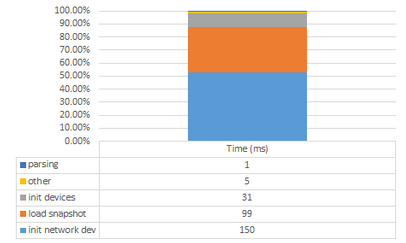
\includegraphics[width=0.4\textwidth]{figs/instantiation.png}
\caption{breakdown of VM instantiation time.}
\end{figure}

The result in figure 1 shows that, instantiating a new VM from scratch can be done within 300 ms. And the main part of instantiation time are network setup and loading snapshot.

\parae{CPU Overhead}


\begin{figure}[H]
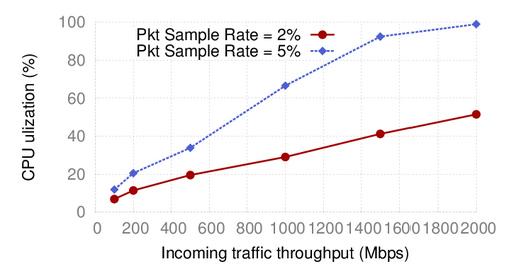
\includegraphics[width=0.4\textwidth]{figs/CPU.png}
\caption{CPU Overhead.}
\end{figure}

%\input{discussion}
%\input{correlation}
%\input{validation}
%\input{implication}
\input{related}
%\input{discussion}
%\input{conclusion}

%\newpage
{\bibliographystyle{abbrv}
\bibliography{reference}}

\end{document}
